\subsection{Rod Cusping Description}
\begin{frame}

\begin{columns}
\begin{column}{0.6\textwidth}
    \begin{itemize}
        \item Nodes must be axially homogeneous
        \item Control rod positions often do not align with node boundaries, 
        requiring homogenization of control rod and moderator
        \item Volume homogenization preserves material volume/mass, but not 
        reaction rates
        \item Two approaches to prevent rod cusping:
        \begin{itemize}
          \item Refine mesh to align with all control rod positions
          \item Decusping method to improve homogenization
        \end{itemize}
    \end{itemize}
\end{column}
\begin{column}{0.4\textwidth}
\begin{figure}[h]
  \centering
  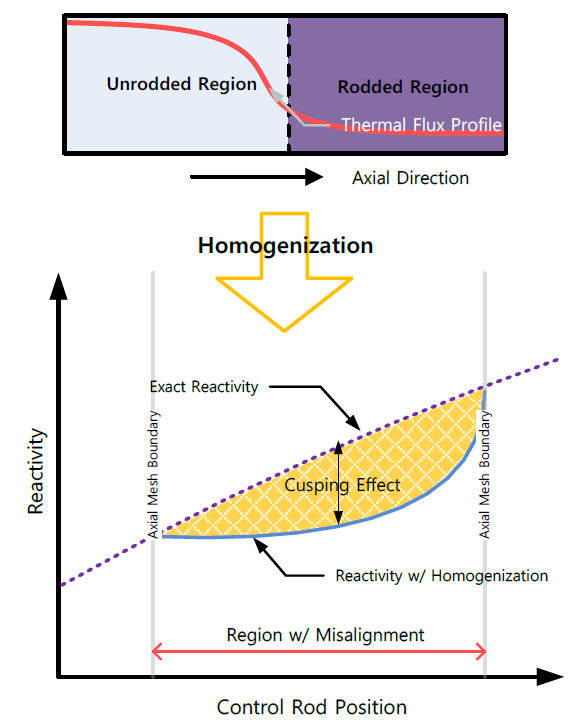
\includegraphics[width=\textwidth]{cusping_effect_Joo.png}
\end{figure} 
\end{column}
\end{columns}
    
\end{frame}

%%%%%%%%%%%%%%%%%%%%%%%%%%%%%%%%%%%%%%%%%%%%%%%%%%%%%%%%%%%%%%%%%%%%%%%%%%%%%%%%%

\begin{frame}
    
    Insert mpact cusping picture here
    
\end{frame}

%%%%%%%%%%%%%%%%%%%%%%%%%%%%%%%%%%%%%%%%%%%%%%%%%%%%%%%%%%%%%%%%%%%%%%%%%%%%%%%%%

\begin{frame}[t]{Methods Shortcomings}
    
    \begin{itemize}
        \item Stuff
    \end{itemize}

\end{frame}